\chapter{Anforderungen}

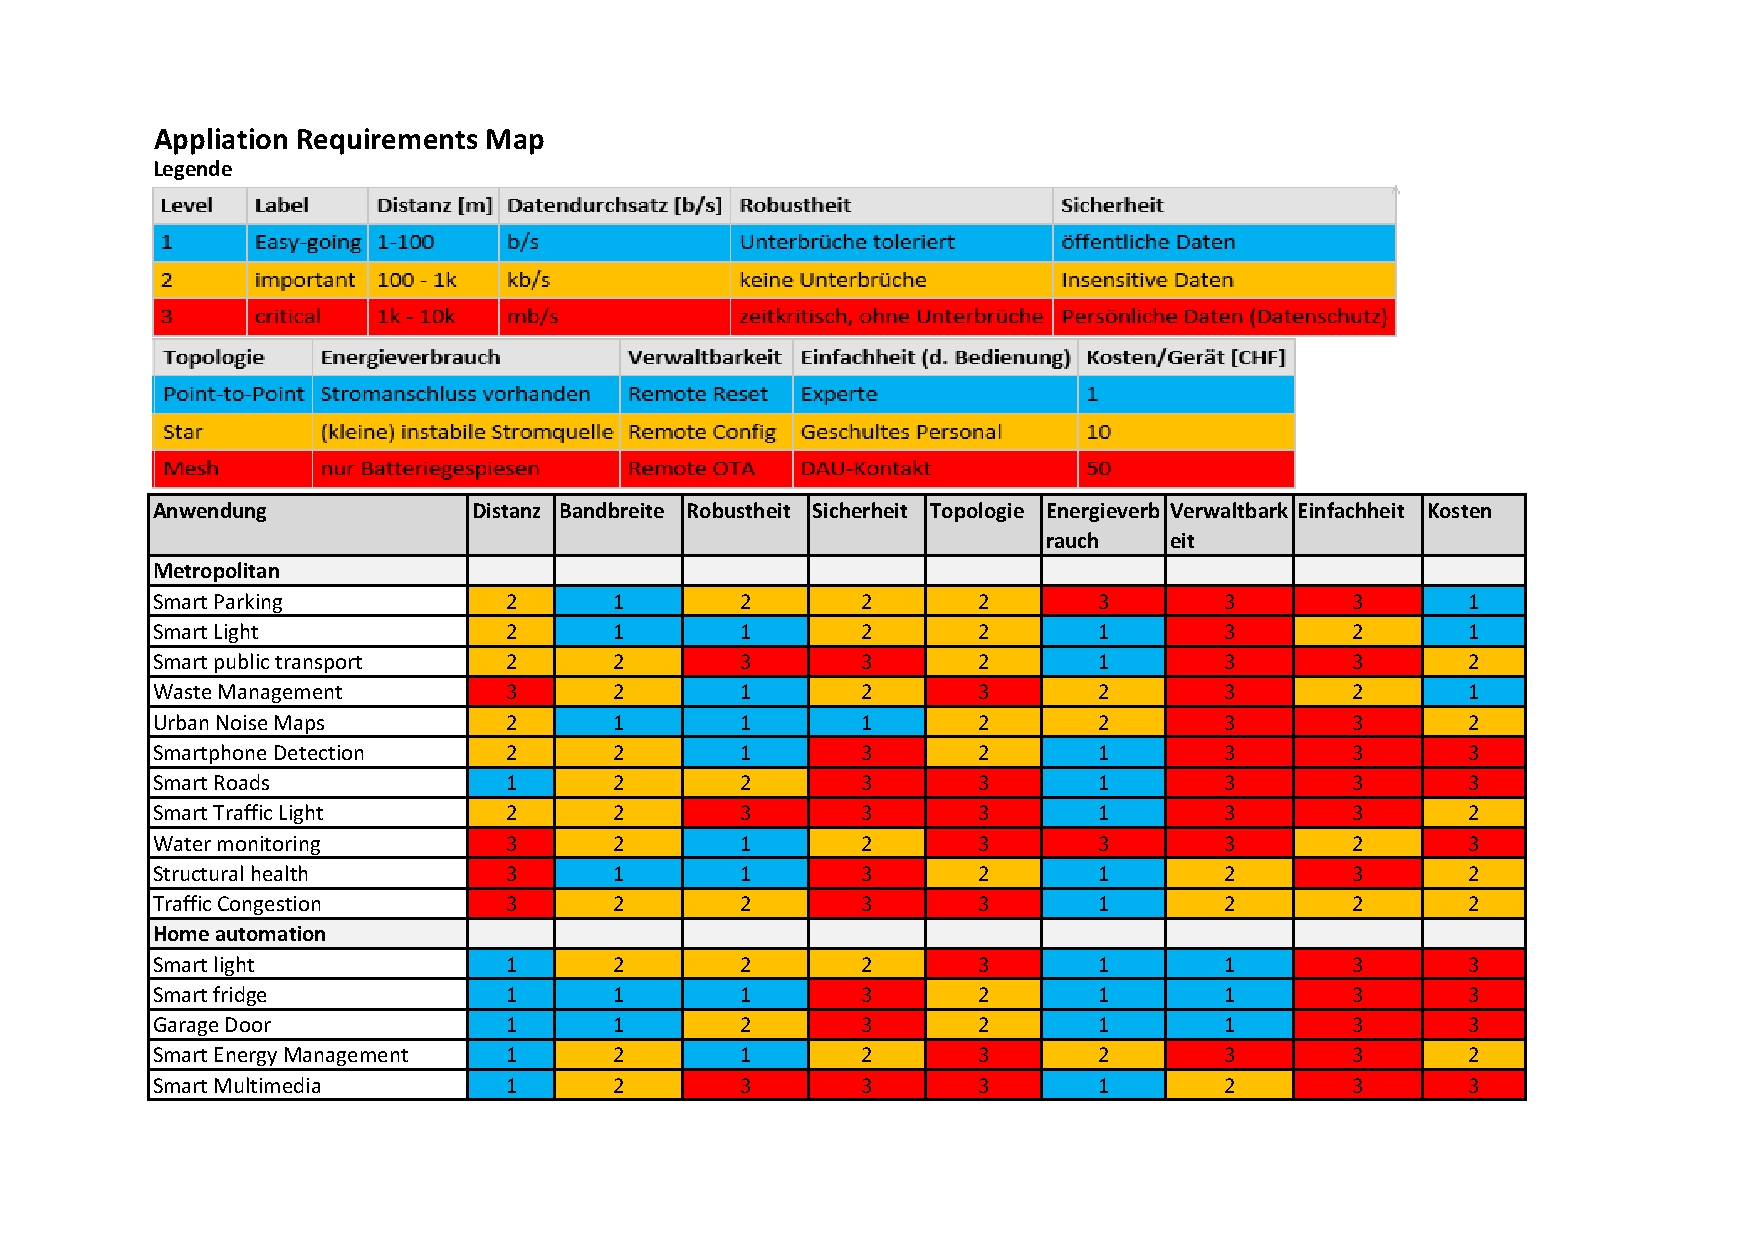
\includepdf[pages=-,landscape,addtotoc={
     1,section,1,Application Requirements Map,p1
}]{appendix/arm.pdf}\label{appendix:arm}

\section{Anforderungen Hardware}

Hardwareanforderungen für den TRESH-Prototype.

\begin{table}[H]
  \centering
  % A table with adjusted row and column spacings
  % \setlength sets the horizontal (column) spacing
  % \arraystretch sets the vertical (row) spacing
  \begingroup
  \setlength{\tabcolsep}{7pt} % Default value: 6pt
  \renewcommand{\arraystretch}{1.4} % Default value: 1
  \begin{tabulary}{1.0\textwidth}{LLLL}
    \rowcolor{LightCyan}
    \rowcolor[HTML]{656565}
    \textbf{ID} & \textbf{Anforderung für Entwickler} & \textbf{Priorität}  & \textbf{Priorität} \\
    \rowcolor[HTML]{9B9B9B}
    1 & Funktionale Anforderungen & Prototype & Produkt \\
    \rowcolor[HTML]{EFEFEF}
    1 & Hardware &  &  \\
    1.1 & \pbox{20cm}{\textbf{SoC (System on a Chip)} \\ Für Energieverbrauchsminimierung soll das System auf einem Chip laufen.} & 3 & 2\\
    1.2 & \pbox{20cm}{\textbf{RTC (Real Time Clock)} \\ Um das System in den Schlafmodus zu bringen und wieder aufzuwecken.} & 1 & 1\\
    1.3 & \pbox{20cm}{\textbf{Funkmodul} \\ 
    - LoRa\\
	- Zigbee\\
	- Sigfox\\
	- Tiny-Mesh\\
	- BLE} & 3 & 2\\
    1.4 & \pbox{20cm}{\textbf{Schnittstellen für Erweiterbarkeit} \\ System hat SPI,  I2C, CANBUS, UART, USB-Schnittstelle} & 2 & 2\\
    1.5 & \pbox{20cm}{\textbf{IO-Ports} \\
    System hat mind.\\
	- 2 Analog In-/Outputs\\
	- 4 Digital In-/Outputs (davon mind. 3 PWM)} & 1 & 1\\

    \rowcolor[HTML]{9B9B9B}
     & Nichtfunktionale Anforderungen & Prototype & Produkt \\
    \rowcolor[HTML]{EFEFEF}
    2 & Funkmodul &  &  \\
    2.1 & \pbox{20cm}{\textbf{OTA} \\ Das System kann Over-The-Air aktualisiert werden.} & 3 & 1\\
    2.2 & \pbox{20cm}{\textbf{Meshing (abhängig von  Radio-Modul)} \\ Das Radio-Modul baut Netzwerk als Mesh-Topologie auf.} & 2 & 1\\
    2.3 & \pbox{20cm}{\textbf{Star (abhängig von  Radio-Modul)} \\ Das Radio-Modul baut Netzwerk als Star-Topologie auf.} & 2 & 2\\
    
    \rowcolor[HTML]{EFEFEF}
    3 & Energie &  &  \\
    3.1 & \pbox{20cm}{\textbf{Energy Management} \\ System hat Sleep-Mode um Energie zu sparen.} & 3 & 1\\
    3.2 & \pbox{20cm}{\textbf{Tiefer Energieverbrauch} \\ System verbraucht im Betrieb maximal 15 mAs.} & 3 & 1\\
    
    \rowcolor[HTML]{EFEFEF}
    4 & Sicherheit &  &  \\
    4.1 & \pbox{20cm}{\textbf{Crypto Chip} \\ Hardware Accelerated Cryptography.} & 3 & 1\\
    
	\rowcolor[HTML]{EFEFEF}
    5 & Entwicklung &  &  \\
    5.1 & \pbox{20cm}{\textbf{Simple Hardware Toolchain} \\ Das Aufspielen von neuer Software soll durch eine Steckverbindung \\ (USB, Steckbare Drähte, \dots)  möglich sein.} & 2 & 1\\
    5.1 & \pbox{20cm}{\textbf{Simple Software Toolchain} \\ Das Aufspielen und Debuggen neuer Software \\ soll über plattformunabhängige Programme möglich sein. Wenn möglich \\ soll dabei Open Source Tools verwendet/unterstützt werden.} & 2 & 1\\
    \bottomrule
  \end{tabulary}
  \endgroup
  \caption{Hardwareanforderungen für einen \gls{iotk}}
  \label{tab:hardwareanforderungen-iotk}
\end{table}


\newpage

\section{Anforderungen Software}

Softwareanforderungen für den TRESH-Prototype.

\begin{table}[H]
  \centering
  % A table with adjusted row and column spacings
  % \setlength sets the horizontal (column) spacing
  % \arraystretch sets the vertical (row) spacing
  \begingroup
  \setlength{\tabcolsep}{7pt} % Default value: 6pt
  \renewcommand{\arraystretch}{1.4} % Default value: 1
  \begin{tabulary}{1.0\textwidth}{LLLL}
    \rowcolor{LightCyan}
    \rowcolor[HTML]{656565}
    \textbf{ID} & \textbf{Anforderung für Entwickler} & \textbf{Priorität}  & \textbf{Priorität} \\
    \rowcolor[HTML]{9B9B9B}
    1 & Funktionale Anforderungen & Prototype & Produkt \\
    \rowcolor[HTML]{EFEFEF}
    1 & Software/Applikation &  &  \\
    1.1 & \pbox{20cm}{\textbf{Messung} \\ System misst den Füllstand des Mülls anhand von Distanz-Sensoren.} & 1 & 1\\
    1.2 & \pbox{20cm}{\textbf{Kalibration} \\ System muss seinen \glqq{}Müll-Füllstand\grqq{} selber kalibrieren können, \\ um Füllstand in \% ausgeben zu können.} & 2 & 1\\
    1.3 & \pbox{20cm}{\textbf{Übertragung der Messdaten} \\ 
Messdaten sollen über eine Wireless-Verbindung an ein IoT-Gateway \\ übermittelt werden.} & 1 & 1\\
    1.4 & \pbox{20cm}{\textbf{Unterstützung verschiedener Wireless Stacks} \\ Die Software muss verschiedene Übertragunsmodule ansteuern können \\ (Modularität).} & 3 & 2\\

    \rowcolor[HTML]{9B9B9B}
     & Nichtfunktionale Anforderungen & Prototype & Produkt \\
    \rowcolor[HTML]{EFEFEF}
    2 & Funkmodul &  &  \\
    2.1 & \pbox{20cm}{\textbf{Kontaktloses Software Update} \\ Neue Software kann ohne jedes Gerät einzeln zu flashen aktualisiert werden.} & 3 & 1\\
    2.2 & \pbox{20cm}{\textbf{Gestaffeltes Software Update} \\ Aktualisierung kann auf definierte Geräte beschränkt werden.} & 3 & 3\\
    2.3 & \pbox{20cm}{\textbf{Geeignete Netzwerk-Topologie} \\ System unterstützt Netzwerk-Topologien wie Mesh- oder Star-Topologie, \\ je nach Anwendungfall.} & 2 & 1\\
    
    \rowcolor[HTML]{EFEFEF}
    3 & Energie &  &  \\
    3.1 & \pbox{20cm}{\textbf{Energy Management} \\ System hat Sleep-Mode um Energie zu sparen.} & 1 & 1\\
    3.2 & \pbox{20cm}{\textbf{Time Sync (RTC)} \\ Das System hat einen RTC für um die Hauptplatine aufzuwecken.} & 1 & 1\\
    3.3 & \pbox{20cm}{\textbf{Lebensdauer} \\ Das System muss mindestens bis zur nächsten Leerung des Mülleimers \\ Energie haben.} & 3 & 1\\
        
    \rowcolor[HTML]{EFEFEF}
    4 & Sicherheit &  &  \\
    4.1 & \pbox{20cm}{\textbf{Radio-Security} \\ Radio-Daten sind (mind.) AES-128 verschlüsselt.} & 3 & 1\\
    4.2 & \pbox{20cm}{\textbf{System-Security} \\ System hat Daten lokal verschlüsselt.} & 3 & 2\\
    \bottomrule
  \end{tabulary}
  \endgroup
  \caption{Softwareanforderungen für einen \gls{iotk}}
  \label{tab:softwareanforderungen-iotk}
\end{table}
